\section{连接杆建模方法分析}\label{sec:lianjieganfenxi}
\subsection{实体建模法}
从图\ref{fig:xiaolunlianjiegan}中可以看出,连接杆由$\phi 14$长6、$\phi 14$长27、$\phi 14$长9、$\phi 18$长3和$\phi 8$长4五段组成的阶梯轴,因此可以分段构建连接杆的实体,最后进组合,其分段实体如图\ref{fig:lianjieganfenxi1}所示。我们把这种应用简单实体进行组合来构建实体模型的方法称之为实体建模法。

\begin{figure}[htbp]
\centering
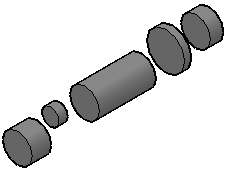
\includegraphics[scale=0.6]{lianjieganfenxi1.png}
\caption{连接杆实体建模}\label{fig:lianjieganfenxi1}
\end{figure}
\subsection{旋转建模法}
图\ref{fig:xiaolunlianjiegan}的连接杆还可以采用旋转法进行建模。所谓旋转建模法是应用能够表征回转体特征的轴向截面,围绕其轴线旋转一周来构建实体模型的方法。旋转建模法只能够用于构建具有回转体结构的模型。图\ref{fig:lianjieganjiemian}为忽略倒角后的截面图,图形是上下对称的结构。从旋转建模法的对特征面定义可知,能够表征连接标杆回转体特征的轴向截面如图\ref{fig:lianjieganduichen}所示。根据前面学习的经验,可以将图\ref{fig:lianjieganduichen}所示的特征截面看作处于同一水平线上的五个不同尺寸的矩形组合而成,其结果如图\ref{fig:lianjieganfenxi2}所示。通过这样的处理,再一次将复杂的图形处理为几个简单的平面图形的组合,减小的构图的难度。
\begin{figure}[htbp]
\begin{floatrow}[3]
\ffigbox{\caption{连接杆截面}\label{fig:lianjieganjiemian}}{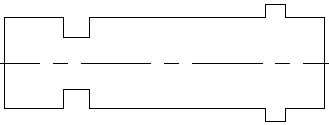
\includegraphics[scale=0.4]{lianjieganjiemian.png}}
\ffigbox{\caption{连接杆特征截面}\label{fig:lianjieganduichen}}{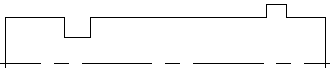
\includegraphics[scale=0.4]{lianjieganduichen.png}}
\ffigbox{\caption{特征截面组合示意}\label{fig:lianjieganfenxi2}}{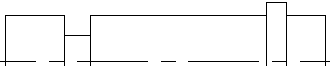
\includegraphics[scale=0.4]{lianjieganfenxi2.png}}
\end{floatrow}
\end{figure}

\yaodian{分析的目的是要从复杂对象中找出构成它的简单对象及组合方式。}
\endinput